\section{Properties of the Benchmark}

\begin{figure*}[h]
\begin{center}
$$ 
\begin{bmatrix}
\frac{1}{2} & -\frac{1}{2} & \frac{1}{2} & -\frac{1}{2} & \frac{1}{2} & -\frac{1}{2}  \\
-\frac{1}{2} & \frac{1}{2} & \frac{1}{2} & -\frac{1}{2} & \frac{1}{2} & -\frac{1}{2} \\
\frac{1}{2} & -\frac{1}{2} & -\frac{1}{2} & \frac{1}{2} & \frac{1}{2} & -\frac{1}{2}  \\
-\frac{1}{2} & \frac{1}{2} & -\frac{1}{2} & \frac{1}{2} & \frac{1}{2} & -\frac{1}{2} \\
\frac{1}{2} & -\frac{1}{2} & \frac{1}{2} & -\frac{1}{2} & -\frac{1}{2} & \frac{1}{2}  \\
-\frac{1}{2} & \frac{1}{2} & \frac{1}{2} & -\frac{1}{2} & -\frac{1}{2} & \frac{1}{2}  \\
\frac{1}{2} & -\frac{1}{2} & -\frac{1}{2} & \frac{1}{2} &-\frac{1}{2} & \frac{1}{2} \\
-\frac{1}{2} & \frac{1}{2} & -\frac{1}{2} & \frac{1}{2}  & -\frac{1}{2} & \frac{1}{2} \\
\end{bmatrix} ~~~~~~~~
% \begin{bmatrix}
% \frac{2}{3} & -\frac{1}{3} & -\frac{1}{3} & \frac{2}{3} & -\frac{1}{3} & -\frac{1}{3}\\
% \frac{2}{3} & -\frac{1}{3} & -\frac{1}{3} & -\frac{1}{3} & \frac{2}{3} & -\frac{1}{3}\\
% \frac{2}{3} & -\frac{1}{3} & -\frac{1}{3} & -\frac{1}{3} & -\frac{1}{3} & \frac{2}{3}\\
%  -\frac{1}{3} & \frac{2}{3} & -\frac{1}{3} & \frac{2}{3} & -\frac{1}{3} & -\frac{1}{3}\\
% -\frac{1}{3} & \frac{2}{3} & -\frac{1}{3} & -\frac{1}{3} & \frac{2}{3} & -\frac{1}{3}\\
% -\frac{1}{3} & \frac{2}{3} &  -\frac{1}{3} & -\frac{1}{3} & -\frac{1}{3} & \frac{2}{3}\\
% -\frac{1}{3} & -\frac{1}{3} & \frac{2}{3} & \frac{2}{3} & -\frac{1}{3} & -\frac{1}{3}\\
% -\frac{1}{3} & -\frac{1}{3} & \frac{2}{3} & -\frac{1}{3} & \frac{2}{3} & -\frac{1}{3}\\
% -\frac{1}{3} & -\frac{1}{3} & \frac{2}{3} & -\frac{1}{3} & -\frac{1}{3} & \frac{2}{3}\\
% \end{bmatrix} 
\begin{bmatrix}
 \frac{2}{3}   & -\frac{1}{3}  & -\frac{1}{3} & \frac{2}{3}   & -\frac{1}{3}  & -\frac{1}{3}   \\
 -\frac{1}{3}  & \frac{2}{3}   & -\frac{1}{3} & \frac{2}{3}   & -\frac{1}{3}  & -\frac{1}{3}   \\
 -\frac{1}{3}  & -\frac{1}{3}  & \frac{2}{3}  & \frac{2}{3}   & -\frac{1}{3}  & -\frac{1}{3}   \\
 \frac{2}{3}   & -\frac{1}{3}  & -\frac{1}{3} & -\frac{1}{3}  & \frac{2}{3}   & -\frac{1}{3}   \\
 -\frac{1}{3}  & \frac{2}{3}   & -\frac{1}{3} & -\frac{1}{3}  & \frac{2}{3}   & -\frac{1}{3}   \\
 -\frac{1}{3}  & -\frac{1}{3}  & \frac{2}{3}  & -\frac{1}{3}  & \frac{2}{3}   &  -\frac{1}{3}  \\
 \frac{2}{3}   & -\frac{1}{3}  & -\frac{1}{3} & -\frac{1}{3}  & -\frac{1}{3}  & \frac{2}{3}    \\
 -\frac{1}{3}  & \frac{2}{3}   & -\frac{1}{3} & -\frac{1}{3}  & -\frac{1}{3}  & \frac{2}{3}    \\
 -\frac{1}{3}  & -\frac{1}{3}  & \frac{2}{3}  & -\frac{1}{3}  & -\frac{1}{3}  & \frac{2}{3}    \\
\end{bmatrix} 
$$
\end{center}
\caption{Benchmark construction for $k=2$ and $\alpha=3$ (left) and $k=3$ and $\alpha=2$ (right).}
\label{fig:benchmark-small-instances}
\end{figure*}


\begin{fact}
For $a\neq a'$, we have $d(\mathcal{C}^{a},\mathcal{C}^{a'}) = 1-1/k$.
\end{fact}
\begin{proof}
Consider an arbitrary vector $v_i^{\ell}$. By construction, the positive entries of $v_i^{\ell}$ range from $k^{\ell-1}\cdot i+1$ to $k^{\ell-1}\cdot (i+1)$. Similarly, the positive entries for the vector $v_j^{\ell-1}$ range from range from $k^{\ell-2}\cdot j+1$ to $k^{\ell-2}\cdot (j+1)$. Therefore, concatenating $v_j^{\ell-1}$ $k$ times into a vector $v'$, $v'$ and $v_i^{\ell}$ can share at most one positive coordinate. Inductively, the same holds true for any concatenation of vectors $v_j^{\ell-h}$.
Thus, the two clusters induced by the columns formed by concatenating the vectors $v$ can share only a $1/k$ fraction of the points. Since each cluster consists of exactly $k^{\alpha}/k$ = $k^{\alpha-1}$ points, the confusion matrix $M$ only has entries $\frac{n}{k^2}$ and for any permutation $\pi$, we have $d(\mathcal{C}^{a},\mathcal{C}^{a'}) = 1-1/k$.
\end{proof}

\begin{fact}
\label{fact:cost}
For any $C_j^a$, we have $\cost_{C_j^a}(\{\mu(C_j^a)\}) = (\alpha-1)\cdot k^{\alpha-2}\cdot (k-1)$.
\end{fact}
\begin{proof}
Without loss of generality, we consider $C_1^0$; the proof is analogous for the other choices of $j$ and $a$. We first note that for any point $A_i \in C_1^0$, the coordinates $A_{i,\ell}$ are identical for $\ell <k$. Furthermore for the column $\ell\geq k$, we have by construction $\sum_{A_i\in C_j} A_{i,\ell} = k^{\alpha-1}\cdot \frac{k-1}{k} + (k^{\alpha}-k^{\alpha-1})\frac{1}{k}=k^{\alpha-1}\cdot (\frac{k-1}{k} - (k-1)\frac{1}{k}) = 0.$ Therefore, the mean of $C_1^0$ satisfies $\mu(C_1^0)_{\ell} = \begin{cases}A_{i,\ell} &\text{if }\ell<k \\
0 &\text{else.}\end{cases}$. 
Thus, the cost is precisely $(\alpha-1)\cdot k^{\alpha-1}\cdot \left(\left(\frac{k-1}{k}\right)^2 + \left(\frac{1}{k}\right)^2 \right)=(\alpha-1)\cdot k^{\alpha-2}\cdot (k-1)$.
\end{proof}

Finally, we show that the means for the clustering $\mathcal{C}^{a}$ also induce $\mathcal{C}^{a}$.

\begin{fact}
\label{fact:opt}
For a clustering $\mathcal{C}^{a}$, let $\mu(C_j^{a})$ denote the mean of cluster $C_j^a$. Then every point  is assigned to its closest center. Moreover, every point $A_i$ of $C_j^a$ has equal distance to any center $\mu(C_h^{a})$ with $h\neq j$.
\end{fact}
\begin{proof}
Again, we assume without loss of generality $a=0$.
Let $A_i$ be an arbitrary point of cluster $C_{h}^{a}$ and consider the mean $\mu(C_j^a)_{\ell} = \begin{cases}A_{i,\ell} &\text{if }\ell<k \\
0 &\text{else.}\end{cases}$ of cluster $C_j^a$. By definition, the positive coordinates of $A_i$ are not equal to the positive coordinates of $\mu(C_j^a)$. The only difference in coordinates between the means of $\mu(C_j^a)$ and $\mu(C_h^a)$ are the first $k$ coordinates, as the rest are $0$.
But here the coordinates of $\mu(C_h^a)$ and $A_i$ are identical, hence $\mu(C_j^a)$ cannot be closer to $A_i$.

To prove that the distances between $A_i$ and any $\mu(C_h^{a})$ with $h\neq j$ are equal, again consider that any difference can only exist among the first $k$ coordinates. Here, we have $\mu(C_h^{a})_h = \frac{k-1}{k}$, and the remaining columns are $-\frac{1}{k}$. Since $A_{i,h} = -\frac{1}{k}$ for any $h\neq j$, the claim follows.
\end{proof}

\section{Hardness of Weak Coreset Evaluation}

Here, we show that it is in general co-NP hard to evaluate whether two point sets $A$ and $B$ are weak coresets of each other. A weak coreset only requires that a $(1+\varepsilon)$ approximation for one point set is a $(1+O(\varepsilon))$ for the other.


\begin{proposition}
\label{prop:hardness}
Given two point sets $A$ and $B$ in $\mathbb{R}^d$ and a sufficiently small (constant) $\varepsilon>0$, it is co-NP hard to decide whether $A$ is a weak coreset of $B$.
\end{proposition}
\begin{proof}
First, we recall that for some $\varepsilon_0$ and candidate clustering cost $V$, it is NP-hard to decide whether there exists a clustering $C$ with cost in $\cost_A(C)\leq V$ and $\cost_B(C)\geq (1+\varepsilon_0)\cdot V$.
Conversely, it is co-NP-hard to decide whether there exists no set of centers $C$ such that $\cost_A(C)\leq V$ and $\cost_B(C) \geq (1+\varepsilon_0)\cdot V$.
\end{proof}

We remark that the possible values for $\varepsilon_0$ are determined by the current APX-hardness results. Assuming NP$\neq$P, $\varepsilon_0\approx 1.07$ and assuming UCG, $\varepsilon_0 \approx 1.17$~\cite{Cohen-AddadSL21,Cohen-AddadS19} for $k$-means in Euclidean spaces.




\section{Distortions}

\begin{longtable}{p{.15\textwidth}lrlllll} 
\toprule 
\parbox[t]{2cm}{\ \\Data set}  & \parbox[t]{5mm}{\ \\$k$} & \parbox[t]{5mm}{\ \\$m$} &           BICO & \parbox[t]{1cm}{Group\\Sampling} &      Ray Maker & \parbox[t]{1cm}{Sensitivity\\Sampling} &    StreamKM++ \\
% Dataset & $k$ &                &                &                &                      &               \\
\midrule
Benchmark & 10  & 50  &   3.40 (0.440) &   1.02 (0.010) &   5.05 (0.157) &         1.02 (0.005) &  1.07 (0.005) \\
      &     & 100 &   3.24 (0.729) &   1.01 (0.004) &   3.84 (0.081) &         1.01 (0.003) &  1.05 (0.004) \\
      &     & 200 &   2.90 (0.153) &   1.01 (0.002) &   3.48 (0.052) &         1.01 (0.002) &  1.04 (0.002) \\
      &     & 500 &   2.62 (0.095) &   1.01 (0.001) &   3.40 (0.058) &         1.00 (0.001) &            \\
% \midrule % light
      & 20  & 50  &   3.22 (0.160) &   1.04 (0.004) &   5.52 (0.266) &         1.02 (0.003) &  1.08 (0.006) \\
      &     & 100 &   3.09 (0.122) &   1.02 (0.004) &   4.31 (0.130) &         1.01 (0.002) &  1.08 (0.003) \\
      &     & 200 &   2.88 (0.078) &   1.01 (0.002) &   3.93 (0.120) &         1.01 (0.001) &  1.11 (0.002) \\
      &     & 500 &   2.36 (0.051) &   1.01 (0.001) &   3.81 (0.116) &         1.01 (0.001) &            \\
% \midrule % light
      & 30  & 50  &   2.81 (0.244) &   1.03 (0.006) &   6.43 (0.470) &         1.02 (0.002) &  1.13 (0.004) \\
      &     & 100 &   2.58 (0.105) &   1.02 (0.003) &   4.65 (0.256) &         1.02 (0.002) &  1.13 (0.004) \\
      &     & 200 &   2.38 (0.098) &   1.01 (0.002) &   4.12 (0.234) &         1.01 (0.002) &  1.10 (0.002) \\
      &     & 500 &   2.01 (0.065) &   1.01 (0.001) &   4.00 (0.138) &         1.01 (0.001) &            \\
% \midrule % light
      & 40  & 50  &   3.16 (0.500) &   1.03 (0.004) &   5.62 (0.287) &         1.02 (0.004) &  1.10 (0.004) \\
      &     & 100 &   2.78 (0.258) &   1.02 (0.001) &   4.42 (0.200) &         1.02 (0.002) &  1.14 (0.003) \\
      &     & 200 &   2.79 (0.217) &   1.02 (0.001) &   3.82 (0.111) &         1.01 (0.001) &  1.17 (0.004) \\
      &     & 500 &   2.57 (0.113) &   1.01 (0.001) &   3.86 (0.122) &         1.01 (0.001) &            \\
\midrule
Caltech & 10  & 50  &   5.12 (0.307) &   1.07 (0.009) &   7.05 (0.250) &         1.05 (0.013) &  1.16 (0.008) \\
      &     & 100 &   4.48 (0.284) &   1.04 (0.006) &   5.46 (0.254) &         1.03 (0.008) &  1.13 (0.005) \\
      &     & 200 &   4.08 (0.319) &   1.02 (0.004) &   5.00 (0.196) &         1.01 (0.005) &  1.10 (0.005) \\
      &     & 500 &   3.41 (0.215) &   1.01 (0.003) &   4.75 (0.188) &         1.00 (0.003) &            \\
% \midrule % light
      & 20  & 50  &   6.35 (1.173) &   1.06 (0.008) &   6.92 (0.209) &         1.05 (0.007) &  1.18 (0.008) \\
      &     & 100 &   4.65 (0.283) &   1.04 (0.005) &   5.29 (0.146) &         1.03 (0.005) &  1.14 (0.005) \\
      &     & 200 &   4.19 (0.384) &   1.02 (0.002) &   4.80 (0.112) &         1.01 (0.004) &  1.12 (0.004) \\
      &     & 500 &   3.50 (0.404) &   1.01 (0.002) &   4.61 (0.096) &         1.00 (0.001) &            \\
% \midrule % light
      & 30  & 50  &   6.01 (0.335) &   1.06 (0.005) &   6.79 (0.149) &         1.04 (0.004) &  1.19 (0.005) \\
      &     & 100 &   5.10 (0.628) &   1.04 (0.005) &   5.30 (0.123) &         1.02 (0.005) &  1.15 (0.002) \\
      &     & 200 &   4.29 (0.659) &   1.02 (0.003) &   4.70 (0.075) &         1.01 (0.003) &  1.13 (0.002) \\
      &     & 500 &   3.09 (0.138) &   1.01 (0.002) &   4.62 (0.090) &         1.00 (0.002) &            \\
% \midrule % light
      & 40  & 50  &   6.24 (0.524) &   1.07 (0.004) &   6.85 (0.145) &         1.05 (0.004) &  1.20 (0.004) \\
      &     & 100 &   5.23 (0.874) &   1.04 (0.003) &   5.22 (0.092) &         1.02 (0.002) &  1.16 (0.003) \\
      &     & 200 &   4.50 (1.085) &   1.02 (0.002) &   4.72 (0.086) &         1.01 (0.001) &  1.13 (0.002) \\
      &     & 500 &   3.38 (0.398) &   1.01 (0.001) &   4.55 (0.094) &         1.00 (0.001) &            \\
% \midrule % light
      & 50  & 50  &   7.50 (1.013) &   1.07 (0.004) &   6.80 (0.092) &         1.05 (0.004) &  1.20 (0.006) \\
      &     & 100 &   5.21 (0.968) &   1.04 (0.003) &   5.18 (0.084) &         1.03 (0.002) &  1.16 (0.005) \\
      &     & 200 &   4.21 (0.296) &   1.02 (0.002) &   4.69 (0.065) &         1.01 (0.003) &  1.13 (0.002) \\
      &     & 500 &   3.36 (0.429) &   1.01 (0.001) &   4.52 (0.058) &         1.00 (0.001) &            \\
\midrule
Caltech+PCA & 10  & 50  &   1.21 (0.009) &   1.03 (0.004) &   1.25 (0.005) &         1.02 (0.007) &  1.04 (0.005) \\
      &     & 100 &   1.19 (0.006) &   1.02 (0.006) &   1.21 (0.006) &         1.01 (0.004) &  1.03 (0.004) \\
      &     & 200 &   1.16 (0.003) &   1.01 (0.002) &   1.19 (0.003) &         1.01 (0.003) &  1.02 (0.002) \\
      &     & 500 &   1.13 (0.007) &   1.00 (0.002) &   1.19 (0.006) &         1.00 (0.001) &            \\
% \midrule % light
      & 20  & 50  &   1.54 (0.024) &   1.04 (0.006) &   1.63 (0.008) &         1.03 (0.006) &  1.07 (0.003) \\
      &     & 100 &   1.48 (0.020) &   1.02 (0.002) &   1.54 (0.010) &         1.01 (0.004) &  1.06 (0.003) \\
      &     & 200 &   1.41 (0.006) &   1.01 (0.002) &   1.50 (0.011) &         1.01 (0.003) &  1.04 (0.003) \\
      &     & 500 &   1.35 (0.008) &   1.00 (0.001) &   1.49 (0.008) &         1.00 (0.001) &            \\
% \midrule % light
      & 30  & 50  &   1.99 (0.032) &   1.05 (0.006) &   2.05 (0.020) &         1.03 (0.003) &  1.10 (0.004) \\
      &     & 100 &   1.82 (0.099) &   1.03 (0.004) &   1.90 (0.014) &         1.02 (0.003) &  1.08 (0.002) \\
      &     & 200 &   1.72 (0.046) &   1.01 (0.002) &   1.84 (0.009) &         1.01 (0.002) &  1.06 (0.002) \\
      &     & 500 &   1.62 (0.037) &   1.01 (0.001) &   1.81 (0.011) &         1.00 (0.002) &            \\
% \midrule % light
      & 40  & 50  &   2.34 (0.112) &   1.05 (0.003) &   2.48 (0.020) &         1.04 (0.005) &  1.12 (0.004) \\
      &     & 100 &   2.25 (0.066) &   1.03 (0.003) &   2.23 (0.011) &         1.02 (0.001) &  1.09 (0.003) \\
      &     & 200 &   2.11 (0.072) &   1.02 (0.002) &   2.15 (0.012) &         1.01 (0.003) &  1.07 (0.002) \\
      &     & 500 &   1.90 (0.070) &   1.01 (0.002) &   2.12 (0.011) &         1.00 (0.001) &            \\
% \midrule % light
      & 50  & 50  &   2.86 (0.214) &   1.06 (0.003) &   2.94 (0.026) &         1.04 (0.005) &  1.14 (0.005) \\
      &     & 100 &   2.58 (0.124) &   1.03 (0.001) &   2.59 (0.019) &         1.02 (0.001) &  1.11 (0.002) \\
      &     & 200 &   2.35 (0.139) &   1.02 (0.001) &   2.49 (0.021) &         1.01 (0.002) &  1.09 (0.002) \\
      &     & 500 &   2.15 (0.075) &   1.01 (0.001) &   2.44 (0.015) &         1.00 (0.001) &            \\
\midrule
Census & 10  & 50  &   2.08 (0.106) &   1.08 (0.019) &   2.30 (0.162) &         1.03 (0.031) &  1.10 (0.012) \\
      &     & 100 &   1.83 (0.124) &   1.04 (0.021) &   1.92 (0.094) &         1.03 (0.012) &  1.07 (0.006) \\
      &     & 200 &   1.65 (0.056) &   1.02 (0.005) &   1.72 (0.050) &         1.02 (0.012) &  1.05 (0.005) \\
      &     & 500 &   1.48 (0.053) &   1.02 (0.004) &   1.69 (0.029) &         1.02 (0.010) &            \\
% \midrule % light
      & 20  & 50  &   2.18 (0.164) &   1.07 (0.022) &   2.31 (0.078) &         1.03 (0.007) &  1.10 (0.008) \\
      &     & 100 &   1.93 (0.080) &   1.04 (0.011) &   1.91 (0.048) &         1.02 (0.011) &  1.08 (0.005) \\
      &     & 200 &   1.71 (0.031) &   1.03 (0.006) &   1.75 (0.027) &         1.01 (0.006) &  1.06 (0.004) \\
      &     & 500 &   1.51 (0.048) &   1.02 (0.005) &   1.66 (0.019) &         1.01 (0.004) &            \\
% \midrule % light
      & 30  & 50  &   2.28 (0.177) &   1.07 (0.011) &   2.38 (0.077) &         1.03 (0.011) &  1.11 (0.007) \\
      &     & 100 &   2.05 (0.096) &   1.04 (0.006) &   1.95 (0.040) &         1.02 (0.007) &  1.09 (0.004) \\
      &     & 200 &   1.76 (0.055) &   1.03 (0.005) &   1.79 (0.034) &         1.01 (0.007) &  1.07 (0.003) \\
      &     & 500 &   1.56 (0.016) &   1.01 (0.003) &   1.71 (0.038) &         1.01 (0.003) &            \\
% \midrule % light
      & 40  & 50  &   2.47 (0.101) &   1.08 (0.009) &   2.43 (0.069) &         1.02 (0.010) &  1.12 (0.006) \\
      &     & 100 &   2.11 (0.104) &   1.04 (0.006) &   1.99 (0.034) &         1.01 (0.004) &  1.09 (0.003) \\
      &     & 200 &   1.83 (0.038) &   1.02 (0.007) &   1.81 (0.026) &         1.01 (0.005) &  1.08 (0.002) \\
      &     & 500 &   1.56 (0.039) &   1.01 (0.005) &   1.73 (0.026) &         1.01 (0.003) &            \\
% \midrule % light
      & 50  & 50  &   2.50 (0.138) &   1.07 (0.008) &   2.48 (0.054) &         1.02 (0.011) &  1.13 (0.004) \\
      &     & 100 &   2.12 (0.109) &   1.04 (0.007) &   2.02 (0.055) &         1.01 (0.004) &  1.10 (0.003) \\
      &     & 200 &   1.84 (0.059) &   1.03 (0.004) &   1.82 (0.022) &         1.01 (0.005) &  1.08 (0.004) \\
      &     & 500 &   1.57 (0.019) &   1.02 (0.004) &   1.75 (0.022) &         1.01 (0.003) &            \\
\midrule
Census+PCA & 10  & 50  &   1.34 (0.048) &   1.06 (0.018) &   1.35 (0.030) &         1.04 (0.021) &  1.03 (0.007) \\
      &     & 100 &   1.24 (0.015) &   1.03 (0.007) &   1.25 (0.017) &         1.03 (0.016) &  1.02 (0.005) \\
      &     & 200 &   1.19 (0.020) &   1.02 (0.009) &   1.19 (0.013) &         1.02 (0.018) &  1.01 (0.002) \\
      &     & 500 &   1.11 (0.003) &   1.01 (0.005) &   1.18 (0.017) &         1.01 (0.003) &            \\
% \midrule % light
      & 20  & 50  &   1.84 (0.118) &   1.07 (0.018) &   1.78 (0.052) &         1.02 (0.012) &  1.07 (0.005) \\
      &     & 100 &   1.57 (0.073) &   1.03 (0.010) &   1.56 (0.020) &         1.02 (0.008) &  1.05 (0.005) \\
      &     & 200 &   1.44 (0.037) &   1.02 (0.007) &   1.44 (0.030) &         1.01 (0.008) &  1.03 (0.002) \\
      &     & 500 &   1.30 (0.014) &   1.01 (0.005) &   1.39 (0.017) &         1.01 (0.005) &            \\
% \midrule % light
      & 30  & 50  &   2.13 (0.153) &   1.07 (0.010) &   2.10 (0.045) &         1.02 (0.011) &  1.10 (0.005) \\
      &     & 100 &   1.81 (0.050) &   1.04 (0.009) &   1.79 (0.029) &         1.01 (0.006) &  1.07 (0.003) \\
      &     & 200 &   1.63 (0.044) &   1.02 (0.006) &   1.65 (0.029) &         1.01 (0.005) &  1.06 (0.002) \\
      &     & 500 &   1.47 (0.021) &   1.01 (0.004) &   1.58 (0.014) &         1.01 (0.004) &            \\
% \midrule % light
      & 40  & 50  &   2.37 (0.102) &   1.07 (0.007) &   2.31 (0.039) &         1.03 (0.008) &  1.11 (0.006) \\
      &     & 100 &   2.01 (0.118) &   1.04 (0.007) &   1.90 (0.027) &         1.01 (0.004) &  1.09 (0.004) \\
      &     & 200 &   1.76 (0.027) &   1.03 (0.005) &   1.75 (0.024) &         1.01 (0.002) &  1.07 (0.002) \\
      &     & 500 &   1.52 (0.044) &   1.02 (0.003) &   1.67 (0.022) &         1.01 (0.003) &            \\
% \midrule % light
      & 50  & 50  &   2.45 (0.139) &   1.07 (0.008) &   2.46 (0.048) &         1.02 (0.012) &  1.13 (0.004) \\
      &     & 100 &   2.14 (0.135) &   1.04 (0.007) &   1.99 (0.028) &         1.01 (0.004) &  1.10 (0.003) \\
      &     & 200 &   1.87 (0.055) &   1.03 (0.005) &   1.82 (0.018) &         1.01 (0.004) &  1.08 (0.002) \\
      &     & 500 &   1.56 (0.008) &   1.02 (0.004) &   1.73 (0.036) &         1.01 (0.004) &            \\
\midrule
Covertype & 10  & 50  &   1.25 (0.018) &   1.08 (0.022) &   1.31 (0.027) &         1.04 (0.025) &  1.05 (0.008) \\
      &     & 100 &   1.17 (0.015) &   1.04 (0.016) &   1.22 (0.017) &         1.03 (0.014) &  1.02 (0.003) \\
      &     & 200 &   1.11 (0.004) &   1.03 (0.012) &   1.18 (0.014) &         1.02 (0.008) &  1.02 (0.002) \\
      &     & 500 &   1.05 (0.001) &   1.01 (0.004) &   1.16 (0.009) &         1.01 (0.006) &            \\
% \midrule % light
      & 20  & 50  &   1.27 (0.025) &   1.09 (0.022) &   1.35 (0.031) &         1.04 (0.008) &  1.05 (0.006) \\
      &     & 100 &   1.18 (0.004) &   1.05 (0.016) &   1.24 (0.010) &         1.02 (0.006) &  1.03 (0.003) \\
      &     & 200 &   1.11 (0.003) &   1.02 (0.008) &   1.21 (0.017) &         1.01 (0.007) &  1.01 (0.002) \\
      &     & 500 &   1.04 (0.001) &   1.01 (0.004) &   1.19 (0.009) &         1.01 (0.006) &            \\
% \midrule % light
      & 30  & 50  &   1.29 (0.008) &   1.08 (0.017) &   1.37 (0.013) &         1.04 (0.013) &  1.05 (0.005) \\
      &     & 100 &   1.17 (0.003) &   1.05 (0.007) &   1.26 (0.013) &         1.01 (0.007) &  1.03 (0.003) \\
      &     & 200 &   1.10 (0.001) &   1.03 (0.009) &   1.21 (0.008) &         1.01 (0.005) &  1.01 (0.001) \\
      &     & 500 &   1.04 (0.000) &   1.01 (0.003) &   1.20 (0.006) &         1.01 (0.003) &            \\
% \midrule % light
      & 40  & 50  &   1.28 (0.009) &   1.09 (0.014) &   1.39 (0.012) &         1.03 (0.013) &  1.05 (0.004) \\
      &     & 100 &   1.18 (0.005) &   1.05 (0.011) &   1.26 (0.009) &         1.02 (0.007) &  1.03 (0.002) \\
      &     & 200 &   1.09 (0.002) &   1.02 (0.003) &   1.22 (0.008) &         1.01 (0.005) &  1.01 (0.001) \\
      &     & 500 &   1.03 (0.000) &   1.01 (0.002) &   1.21 (0.008) &         1.01 (0.003) &            \\
% \midrule % light
      & 50  & 50  &   1.28 (0.009) &   1.08 (0.007) &   1.38 (0.008) &         1.03 (0.010) &  1.05 (0.004) \\
      &     & 100 &   1.15 (0.003) &   1.05 (0.005) &   1.27 (0.011) &         1.02 (0.005) &  1.02 (0.001) \\
      &     & 200 &   1.07 (0.001) &   1.02 (0.004) &   1.23 (0.009) &         1.01 (0.002) &  1.01 (0.001) \\
      &     & 500 &   1.03 (0.000) &   1.01 (0.004) &   1.23 (0.009) &         1.01 (0.004) &            \\
\midrule
Covertype+PCA & 10  & 50  &   1.26 (0.024) &   1.09 (0.025) &   1.30 (0.019) &         1.04 (0.017) &  1.04 (0.008) \\
      &     & 100 &   1.16 (0.010) &   1.05 (0.017) &   1.22 (0.015) &         1.03 (0.017) &  1.02 (0.003) \\
      &     & 200 &   1.10 (0.003) &   1.03 (0.017) &   1.17 (0.014) &         1.02 (0.011) &  1.01 (0.002) \\
      &     & 500 &   1.06 (0.001) &   1.01 (0.006) &   1.16 (0.008) &         1.01 (0.007) &            \\
% \midrule % light
      & 20  & 50  &   1.27 (0.018) &   1.10 (0.021) &   1.34 (0.021) &         1.04 (0.018) &  1.05 (0.004) \\
      &     & 100 &   1.17 (0.005) &   1.05 (0.011) &   1.25 (0.013) &         1.02 (0.010) &  1.03 (0.002) \\
      &     & 200 &   1.11 (0.003) &   1.02 (0.007) &   1.20 (0.012) &         1.02 (0.005) &  1.01 (0.002) \\
      &     & 500 &   1.04 (0.001) &   1.01 (0.004) &   1.19 (0.011) &         1.01 (0.008) &            \\
% \midrule % light
      & 30  & 50  &   1.29 (0.010) &   1.09 (0.013) &   1.38 (0.013) &         1.04 (0.011) &  1.05 (0.003) \\
      &     & 100 &   1.17 (0.004) &   1.05 (0.011) &   1.26 (0.009) &         1.01 (0.007) &  1.03 (0.003) \\
      &     & 200 &   1.10 (0.002) &   1.03 (0.005) &   1.22 (0.011) &         1.01 (0.007) &  1.01 (0.002) \\
      &     & 500 &   1.04 (0.000) &   1.01 (0.003) &   1.21 (0.010) &         1.01 (0.005) &            \\
% \midrule % light
      & 40  & 50  &   1.28 (0.006) &   1.09 (0.013) &   1.38 (0.019) &         1.04 (0.014) &  1.05 (0.005) \\
      &     & 100 &   1.18 (0.003) &   1.05 (0.008) &   1.27 (0.016) &         1.02 (0.008) &  1.02 (0.002) \\
      &     & 200 &   1.09 (0.001) &   1.02 (0.004) &   1.22 (0.010) &         1.01 (0.004) &  1.01 (0.002) \\
      &     & 500 &   1.03 (0.000) &   1.01 (0.003) &   1.21 (0.009) &         1.01 (0.003) &            \\
% \midrule % light
      & 50  & 50  &   1.29 (0.017) &   1.09 (0.014) &   1.39 (0.009) &         1.03 (0.010) &  1.05 (0.003) \\
      &     & 100 &   1.15 (0.003) &   1.05 (0.007) &   1.27 (0.009) &         1.02 (0.008) &  1.02 (0.001) \\
      &     & 200 &   1.07 (0.001) &   1.02 (0.003) &   1.22 (0.005) &         1.01 (0.002) &  1.01 (0.001) \\
      &     & 500 &   1.03 (0.000) &   1.01 (0.002) &   1.23 (0.006) &         1.01 (0.003) &            \\
\midrule
NYTimes & 10  & 50  &  35.32 (8.376) &   1.08 (0.009) &  28.37 (2.761) &         1.05 (0.012) &  2.04 (0.244) \\
      &     & 100 &  24.50 (5.355) &   1.06 (0.008) &  17.64 (0.561) &         1.03 (0.007) &  1.80 (0.069) \\
      &     & 200 &  13.97 (2.143) &   1.04 (0.004) &  15.17 (0.512) &         1.02 (0.008) &  1.75 (0.110) \\
      &     & 500 &   8.09 (1.241) &   1.03 (0.004) &  14.16 (1.031) &         1.01 (0.004) &            \\
% \midrule % light
      & 20  & 50  &  21.70 (3.965) &   1.09 (0.008) &  23.94 (1.466) &         1.05 (0.010) &  1.97 (0.083) \\
      &     & 100 &  16.00 (3.906) &   1.05 (0.005) &  14.56 (0.846) &         1.03 (0.006) &  1.79 (0.046) \\
      &     & 200 &   8.64 (1.429) &   1.04 (0.003) &  12.71 (0.786) &         1.02 (0.003) &  1.68 (0.025) \\
      &     & 500 &   5.39 (0.441) &   1.02 (0.001) &  11.73 (0.551) &         1.01 (0.003) &            \\
% \midrule % light
      & 30  & 50  &  21.63 (3.611) &   1.09 (0.007) &  20.44 (0.862) &         1.05 (0.008) &  1.97 (0.106) \\
      &     & 100 &  13.36 (3.778) &   1.05 (0.005) &  13.00 (0.763) &         1.03 (0.005) &  1.74 (0.035) \\
      &     & 200 &   7.76 (0.884) &   1.03 (0.003) &  11.68 (0.754) &         1.01 (0.004) &  1.66 (0.028) \\
      &     & 500 &   4.70 (0.418) &   1.02 (0.001) &  11.17 (0.682) &         1.01 (0.002) &            \\
% \midrule % light
      & 40  & 50  &  22.03 (7.691) &   1.08 (0.006) &  18.56 (0.955) &         1.05 (0.006) &  1.92 (0.045) \\
      &     & 100 &  10.49 (1.801) &   1.05 (0.006) &  12.27 (0.688) &         1.03 (0.006) &  1.75 (0.057) \\
      &     & 200 &   6.39 (0.339) &   1.03 (0.002) &  11.08 (0.461) &         1.01 (0.005) &  1.63 (0.024) \\
      &     & 500 &   4.19 (0.151) &   1.02 (0.001) &  10.68 (0.736) &         1.01 (0.002) &            \\
% \midrule % light
      & 50  & 50  &  15.78 (3.123) &   1.09 (0.005) &  17.61 (0.940) &         1.05 (0.007) &  1.89 (0.053) \\
      &     & 100 &   9.85 (2.053) &   1.05 (0.004) &  11.71 (0.292) &         1.03 (0.003) &  1.71 (0.036) \\
      &     & 200 &   6.03 (0.505) &   1.03 (0.002) &  10.76 (0.454) &         1.01 (0.004) &  1.63 (0.020) \\
      &     & 500 &   4.07 (0.182) &   1.02 (0.001) &  10.58 (1.080) &         1.00 (0.002) &            \\
\midrule
NYTimes+PCA & 10  & 50  &   1.02 (0.002) &   1.01 (0.002) &   1.02 (0.001) &         1.00 (0.002) &  1.00 (0.000) \\
      &     & 100 &   1.01 (0.001) &   1.00 (0.001) &   1.01 (0.001) &         1.00 (0.002) &  1.00 (0.000) \\
      &     & 200 &   1.01 (0.000) &   1.00 (0.001) &   1.01 (0.000) &         1.00 (0.001) &  1.00 (0.000) \\
      &     & 500 &   1.01 (0.000) &   1.00 (0.001) &   1.01 (0.001) &         1.00 (0.001) &            \\
% \midrule % light
      & 20  & 50  &   1.03 (0.002) &   1.01 (0.001) &   1.03 (0.001) &         1.00 (0.002) &  1.01 (0.001) \\
      &     & 100 &   1.03 (0.001) &   1.00 (0.001) &   1.03 (0.001) &         1.00 (0.000) &  1.01 (0.000) \\
      &     & 200 &   1.02 (0.001) &   1.00 (0.001) &   1.02 (0.001) &         1.00 (0.001) &  1.01 (0.000) \\
      &     & 500 &   1.01 (0.001) &   1.00 (0.000) &   1.02 (0.001) &         1.00 (0.000) &            \\
% \midrule % light
      & 30  & 50  &   1.04 (0.003) &   1.01 (0.001) &   1.04 (0.001) &         1.00 (0.002) &  1.02 (0.001) \\
      &     & 100 &   1.04 (0.002) &   1.01 (0.001) &   1.03 (0.001) &         1.00 (0.001) &  1.01 (0.000) \\
      &     & 200 &   1.03 (0.001) &   1.00 (0.001) &   1.03 (0.000) &         1.00 (0.001) &  1.01 (0.000) \\
      &     & 500 &   1.02 (0.000) &   1.00 (0.000) &   1.03 (0.001) &         1.00 (0.001) &            \\
% \midrule % light
      & 40  & 50  &   1.06 (0.001) &   1.01 (0.001) &   1.05 (0.001) &         1.00 (0.001) &  1.02 (0.000) \\
      &     & 100 &   1.05 (0.002) &   1.01 (0.001) &   1.05 (0.001) &         1.00 (0.001) &            \\
      &     & 200 &   1.04 (0.001) &   1.00 (0.001) &   1.04 (0.001) &         1.00 (0.001) &  1.01 (0.000) \\
      &     & 500 &   1.03 (0.000) &   1.00 (0.000) &   1.05 (0.001) &         1.00 (0.000) &            \\
% \midrule % light
      & 50  & 50  &   1.07 (0.004) &   1.01 (0.001) &   1.06 (0.002) &         1.00 (0.001) &            \\
      &     & 100 &   1.06 (0.001) &   1.01 (0.001) &   1.05 (0.001) &         1.00 (0.001) &  1.02 (0.000) \\
      &     & 200 &   1.04 (0.003) &   1.00 (0.001) &   1.05 (0.001) &         1.00 (0.001) &  1.02 (0.000) \\
      &     & 500 &   1.03 (0.001) &   1.00 (0.000) &   1.06 (0.001) &         1.00 (0.000) &            \\
\midrule
Tower & 20  & 50  &   1.18 (0.018) &   1.09 (0.025) &   1.44 (0.045) &         1.04 (0.025) &  1.04 (0.004) \\
      &     & 100 &   1.11 (0.005) &   1.05 (0.016) &   1.16 (0.013) &         1.03 (0.007) &  1.03 (0.003) \\
      &     & 200 &   1.06 (0.002) &   1.03 (0.007) &   1.06 (0.007) &         1.02 (0.009) &  1.02 (0.001) \\
      &     & 500 &   1.03 (0.001) &   1.01 (0.006) &   1.03 (0.002) &         1.01 (0.005) &            \\
% \midrule % light
      & 40  & 50  &   1.20 (0.012) &   1.11 (0.014) &   1.48 (0.020) &         1.04 (0.019) &  1.05 (0.002) \\
      &     & 100 &   1.11 (0.006) &   1.05 (0.013) &   1.15 (0.008) &         1.02 (0.010) &  1.03 (0.002) \\
      &     & 200 &   1.07 (0.005) &   1.03 (0.007) &   1.05 (0.004) &         1.01 (0.006) &  1.02 (0.001) \\
      &     & 500 &   1.02 (0.001) &   1.01 (0.003) &   1.03 (0.001) &         1.01 (0.003) &            \\
% \midrule % light
      & 60  & 50  &   1.20 (0.008) &   1.11 (0.011) &   1.49 (0.019) &         1.04 (0.009) &  1.05 (0.002) \\
      &     & 100 &   1.10 (0.002) &   1.06 (0.007) &   1.13 (0.005) &         1.01 (0.006) &  1.03 (0.002) \\
      &     & 200 &   1.06 (0.002) &   1.03 (0.007) &   1.05 (0.002) &         1.01 (0.004) &  1.02 (0.001) \\
      &     & 500 &   1.02 (0.001) &   1.02 (0.005) &   1.03 (0.001) &         1.01 (0.003) &            \\
% \midrule % light
      & 80  & 50  &   1.18 (0.005) &   1.11 (0.010) &   1.47 (0.013) &         1.03 (0.012) &  1.05 (0.004) \\
      &     & 100 &   1.10 (0.009) &   1.06 (0.008) &   1.13 (0.004) &         1.01 (0.005) &  1.03 (0.001) \\
      &     & 200 &   1.05 (0.001) &   1.03 (0.003) &   1.05 (0.002) &         1.01 (0.004) &  1.02 (0.000) \\
      &     & 500 &   1.02 (0.001) &   1.02 (0.003) &   1.02 (0.001) &         1.01 (0.004) &            \\
% \midrule % light
      & 100 & 50  &   1.19 (0.007) &   1.10 (0.009) &   1.45 (0.010) &         1.03 (0.008) &  1.05 (0.002) \\
      &     & 100 &   1.10 (0.008) &   1.06 (0.007) &   1.12 (0.005) &         1.02 (0.007) &  1.03 (0.001) \\
      &     & 200 &   1.04 (0.001) &   1.03 (0.005) &   1.05 (0.002) &         1.01 (0.003) &  1.02 (0.000) \\
      &     & 500 &   1.01 (0.001) &   1.02 (0.003) &   1.03 (0.002) &         1.01 (0.003) &            \\
\bottomrule
\caption{Distortions of the evaluation algorithms on all data sets with and without PCA preprocessing. Each cell specify the mean distortion along with the standard deviation in parenthesis of 10 repetition of the experiment.}
\label{tab:distortions-mean-std}
\end{longtable}




\begin{longtable}{llrlll} 
\toprule
\parbox[t]{2cm}{Data set} & \parbox[t]{5mm}{$k$} & \parbox[t]{5mm}{$m$} &  \parbox[t]{2cm}{$k$-means++} &  \parbox[t]{2.5cm}{Random CH} &    \parbox[t]{2cm}{Random MEB} \\ 
% Dataset & $k$ &                &                &                &                      &               \\
\midrule
Caltech  & 10 &     50 & 5.12 (0.307) & 4.30 (0.270) &  2.63 (0.166) \\
      &    &    100 & 4.48 (0.284) & 3.91 (0.240) &  2.54 (0.125) \\
      &    &    200 & 4.08 (0.319) & 3.54 (0.236) &  2.46 (0.134) \\
      &    &    500 & 3.41 (0.215) & 3.06 (0.155) &  2.18 (0.080) \\
\midrule
Caltech  & 20 &     50 & 6.35 (1.173) & 4.73 (0.632) &  2.63 (0.147) \\
      &    &    100 & 4.65 (0.283) & 3.82 (0.245) &  2.41 (0.104) \\
      &    &    200 & 4.19 (0.384) & 3.49 (0.271) &  2.26 (0.141) \\
      &    &    500 & 3.50 (0.404) & 3.07 (0.301) &  2.10 (0.128) \\
\midrule
Caltech & 30 &     50 & 6.01 (0.335) & 4.32 (0.204) &  2.57 (0.096) \\
      &    &    100 & 5.10 (0.628) & 3.89 (0.340) &  2.35 (0.125) \\
      &    &    200 & 4.29 (0.659) & 3.47 (0.440) &  2.21 (0.170) \\
      &    &    500 & 3.09 (0.138) & 2.69 (0.122) &  1.87 (0.064) \\
\midrule
Caltech & 40 &     50 & 6.24 (0.524) & 4.33 (0.228) &  2.44 (0.076) \\
      &    &    100 & 5.23 (0.874) & 3.86 (0.434) &  2.29 (0.191) \\
      &    &    200 & 4.50 (1.085) & 3.49 (0.595) &  2.16 (0.183) \\
      &    &    500 & 3.38 (0.398) & 2.85 (0.258) &  1.92 (0.111) \\
\midrule
Caltech & 50 &     50 & 7.50 (1.013) & 4.80 (0.449) &  2.47 (0.190) \\
      &    &    100 & 5.21 (0.968) & 3.76 (0.475) &  2.20 (0.149) \\
      &    &    200 & 4.21 (0.296) & 3.35 (0.195) &  2.10 (0.065) \\
      &    &    500 & 3.36 (0.429) & 2.81 (0.288) &  1.86 (0.105) \\
\bottomrule

\caption{The effect of three solution generation methods on the distortions (see \cref{sec:evaluation-procedure}). We compared generating candidate solutions by running $k$-means++, randomly generating $k$ points inside the convex hull (Random CH) and inside the minimum enclosing ball (Random MEB). Our experiments show that the $k$-means++ method generates candidate solutions which consistently lead to large distortions on all algorithms. Notice that this table only shows the distortions obtained by BICO on the \textit{Caltech} data set.}
\label{tab:comparison-solution-generation}
\end{longtable}




% \begin{longtable}{p{.20\textwidth}llllll} 
% \toprule
% \parbox[t]{2cm}{\ \\Data set}  & \parbox[t]{5mm}{\ \\$k$} &           BICO & \parbox[t]{1cm}{Group\\Sampling} &      Ray Maker & \parbox[t]{1cm}{Sensitivity\\Sampling} &    StreamKM++ \\
% % Dataset & $k$ &                &                &                &                      &               \\
% \midrule % light
% Benchmark & 10  &   2.93 (0.144) &   1.01 (0.002) &   3.49 (0.055) &         1.02 (0.003) &  1.04 (0.002) \\
%       & 20  &   2.87 (0.137) &   1.01 (0.002) &   3.90 (0.112) &         1.02 (0.003) &  1.11 (0.002) \\
%       & 30  &   2.34 (0.070) &   1.02 (0.001) &   4.19 (0.137) &         1.02 (0.002) &  1.10 (0.002) \\
%       & 40  &   2.68 (0.230) &   1.02 (0.001) &   3.83 (0.172) &         1.02 (0.002) &  1.17 (0.004) \\
% \midrule % light
% Caltech & 10  &   4.15 (0.485) &   1.02 (0.003) &   4.99 (0.124) &         1.01 (0.004) &  1.10 (0.004) \\
%       & 20  &   4.16 (0.708) &   1.02 (0.003) &   4.86 (0.134) &         1.01 (0.003) &  1.12 (0.004) \\
%       & 30  &   4.15 (0.416) &   1.02 (0.001) &   4.78 (0.117) &         1.01 (0.002) &  1.13 (0.003) \\
%       & 40  &   4.18 (0.486) &   1.02 (0.002) &   4.73 (0.068) &         1.01 (0.002) &  1.13 (0.001) \\
%       & 50  &   3.99 (0.560) &   1.02 (0.002) &   4.72 (0.090) &         1.01 (0.002) &  1.13 (0.002) \\
% \midrule % light
% Census & 10  &   1.65 (0.082) &   1.03 (0.011) &   1.74 (0.044) &         1.02 (0.006) &  1.05 (0.005) \\
%       & 20  &   1.74 (0.054) &   1.02 (0.004) &   1.75 (0.038) &         1.01 (0.005) &  1.06 (0.003) \\
%       & 30  &   1.77 (0.063) &   1.02 (0.003) &   1.79 (0.032) &         1.01 (0.005) &  1.07 (0.002) \\
%       & 40  &   1.83 (0.038) &   1.02 (0.002) &   1.81 (0.021) &         1.01 (0.005) &  1.08 (0.003) \\
%       & 50  &   1.87 (0.088) &   1.02 (0.002) &   1.85 (0.044) &         1.01 (0.003) &  1.10 (0.059) \\
% \midrule % light
% Covertype & 10  &   1.10 (0.002) &   1.03 (0.011) &   1.18 (0.016) &         1.02 (0.007) &  1.01 (0.002) \\
%       & 20  &   1.11 (0.004) &   1.03 (0.010) &   1.21 (0.015) &         1.01 (0.007) &  1.01 (0.002) \\
%       & 30  &   1.10 (0.003) &   1.03 (0.005) &   1.22 (0.008) &         1.01 (0.005) &  1.01 (0.002) \\
%       & 40  &   1.09 (0.001) &   1.03 (0.005) &   1.22 (0.012) &         1.01 (0.005) &  1.01 (0.001) \\
%       & 50  &   1.07 (0.001) &   1.03 (0.003) &   1.22 (0.008) &         1.01 (0.002) &  1.01 (0.001) \\
% \midrule % light
% NYTimes & 10  &  18.59 (5.356) &   1.04 (0.003) &  15.37 (0.740) &         1.02 (0.004) &  1.75 (0.105) \\
%       & 20  &   9.98 (1.559) &   1.04 (0.003) &  12.71 (0.448) &         1.01 (0.004) &  1.69 (0.024) \\
%       & 30  &   8.03 (2.156) &   1.04 (0.002) &  12.18 (0.974) &         1.02 (0.003) &  1.66 (0.030) \\
%       & 40  &   6.31 (0.436) &   1.03 (0.003) &  11.20 (0.742) &         1.01 (0.002) &  1.63 (0.024) \\
%       & 50  &   5.97 (0.381) &   1.03 (0.002) &  10.81 (0.571) &         1.01 (0.002) &  1.63 (0.026) \\
% \midrule % light
% Tower & 20  &   1.07 (0.003) &   1.02 (0.007) &   1.06 (0.004) &         1.03 (0.009) &  1.02 (0.001) \\
%       & 40  &   1.06 (0.004) &   1.02 (0.006) &   1.06 (0.002) &         1.02 (0.007) &  1.02 (0.001) \\
%       & 60  &   1.06 (0.001) &   1.03 (0.004) &   1.05 (0.004) &         1.01 (0.003) &  1.02 (0.001) \\
%       & 80  &   1.05 (0.001) &   1.03 (0.005) &   1.05 (0.002) &         1.01 (0.006) &  1.02 (0.001) \\
%       & 100 &   1.04 (0.002) &   1.03 (0.004) &   1.05 (0.001) &         1.01 (0.004) &  1.02 (0.001) \\
% \midrule % light
% Caltech+PCA & 10  &   1.16 (0.004) &   1.01 (0.002) &   1.19 (0.009) &         1.00 (0.001) &  1.02 (0.002) \\
%       & 20  &   1.42 (0.016) &   1.01 (0.002) &   1.51 (0.008) &         1.01 (0.001) &  1.04 (0.002) \\
%       & 30  &   1.73 (0.045) &   1.02 (0.001) &   1.83 (0.014) &         1.01 (0.001) &  1.06 (0.002) \\
%       & 40  &   2.13 (0.083) &   1.02 (0.002) &   2.16 (0.016) &         1.01 (0.002) &  1.07 (0.002) \\
%       & 50  &   2.38 (0.139) &   1.02 (0.001) &   2.49 (0.017) &         1.01 (0.002) &  1.09 (0.002) \\
% \midrule % light
% Census+PCA & 10  &   1.18 (0.012) &   1.01 (0.005) &   1.20 (0.016) &         1.02 (0.009) &  1.01 (0.002) \\
%       & 20  &   1.44 (0.046) &   1.02 (0.003) &   1.45 (0.019) &         1.02 (0.010) &  1.04 (0.002) \\
%       & 30  &   1.64 (0.044) &   1.02 (0.004) &   1.63 (0.021) &         1.01 (0.007) &  1.06 (0.003) \\
%       & 40  &   1.77 (0.035) &   1.02 (0.002) &   1.76 (0.028) &         1.01 (0.004) &  1.07 (0.002) \\
%       & 50  &   1.87 (0.068) &   1.02 (0.002) &   1.82 (0.017) &         1.01 (0.004) &  1.08 (0.002) \\
% \midrule % light
% Covertype+PCA & 10  &   1.11 (0.003) &   1.03 (0.012) &   1.19 (0.011) &         1.02 (0.010) &  1.02 (0.002) \\
%       & 20  &   1.11 (0.003) &   1.03 (0.006) &   1.21 (0.010) &         1.02 (0.007) &  1.02 (0.002) \\
%       & 30  &   1.10 (0.002) &   1.03 (0.007) &   1.22 (0.011) &         1.01 (0.005) &  1.01 (0.002) \\
%       & 40  &   1.09 (0.002) &   1.03 (0.006) &   1.23 (0.010) &         1.01 (0.005) &  1.01 (0.001) \\
%       & 50  &   1.07 (0.001) &   1.03 (0.003) &   1.23 (0.008) &         1.01 (0.003) &  1.01 (0.001) \\
% \midrule % light
% NYTimes+PCA & 10  &   1.01 (0.000) &   1.00 (0.000) &   1.01 (0.001) &         1.00 (0.000) &  1.00 (0.000) \\
%       & 20  &   1.02 (0.000) &   1.00 (0.000) &   1.02 (0.001) &         1.00 (0.000) &  1.01 (0.000) \\
%       & 30  &   1.03 (0.000) &   1.00 (0.000) &   1.03 (0.001) &         1.00 (0.000) &  1.01 (0.000) \\
%       & 40  &   1.04 (0.001) &   1.00 (0.000) &   1.04 (0.001) &         1.00 (0.002) &  1.01 (0.000) \\
%       & 50  &   1.04 (0.002) &   1.00 (0.000) &   1.05 (0.001) &         1.00 (0.000) &  1.02 (0.000) \\
% \bottomrule
% \caption{Distortions of the evaluation algorithms on all data sets with and without PCA preprocessing. Each cell specify the mean distortion along with the standard deviation in brackets of 10 repetition of the experiment.}
% \label{tab:distortions-mean-std}
% \end{longtable}











\section{Auxiliary Plots}


\begin{figure}[h!t]
  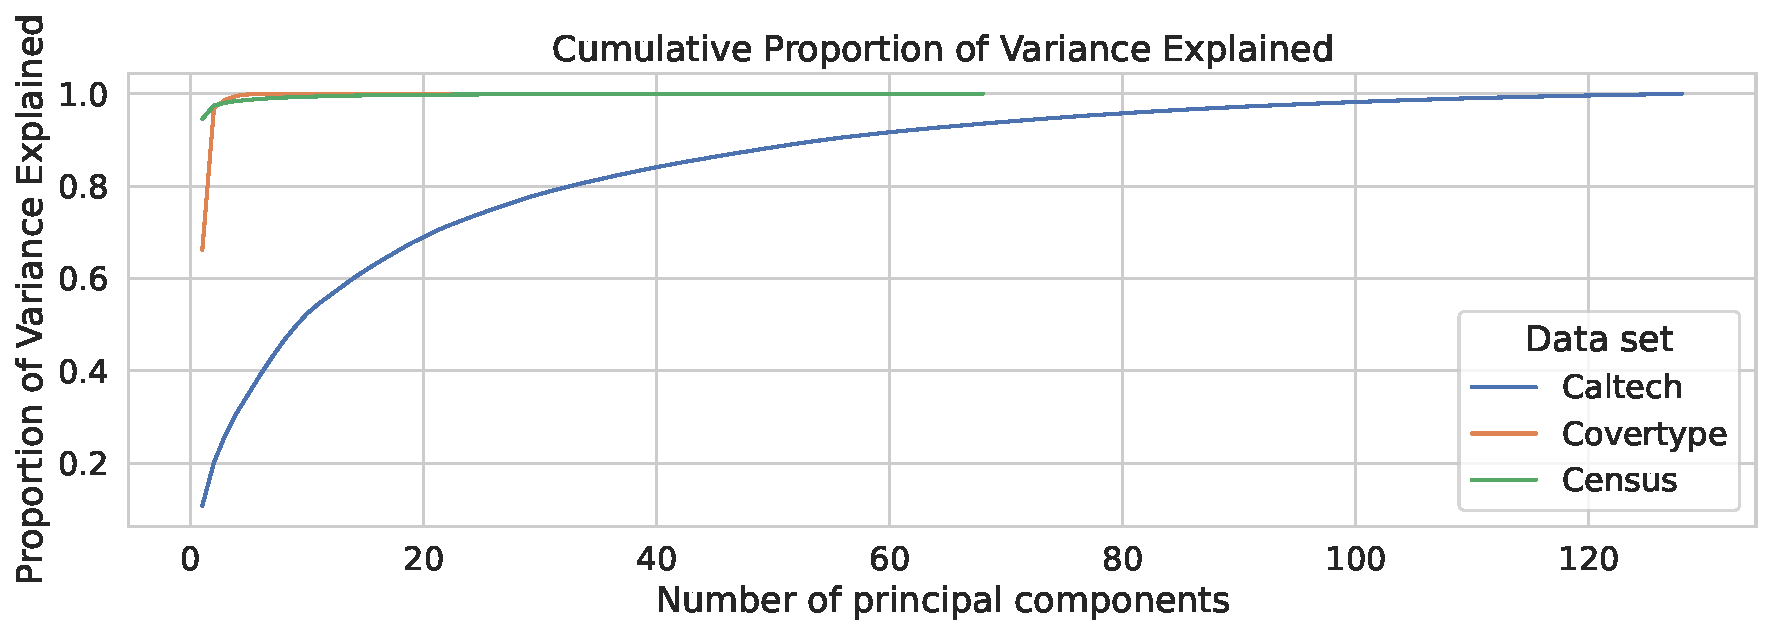
\includegraphics[width=0.9\linewidth]{figures/explained-variance-plot.pdf}
  \caption{The cumulative proportion of explained variance by principal components on \textit{Caltech}, \textit{Covertype}, and \textit{Census}.}
  \label{fig:explained-variance-pca}
\end{figure}

\begin{figure}[!ht]
  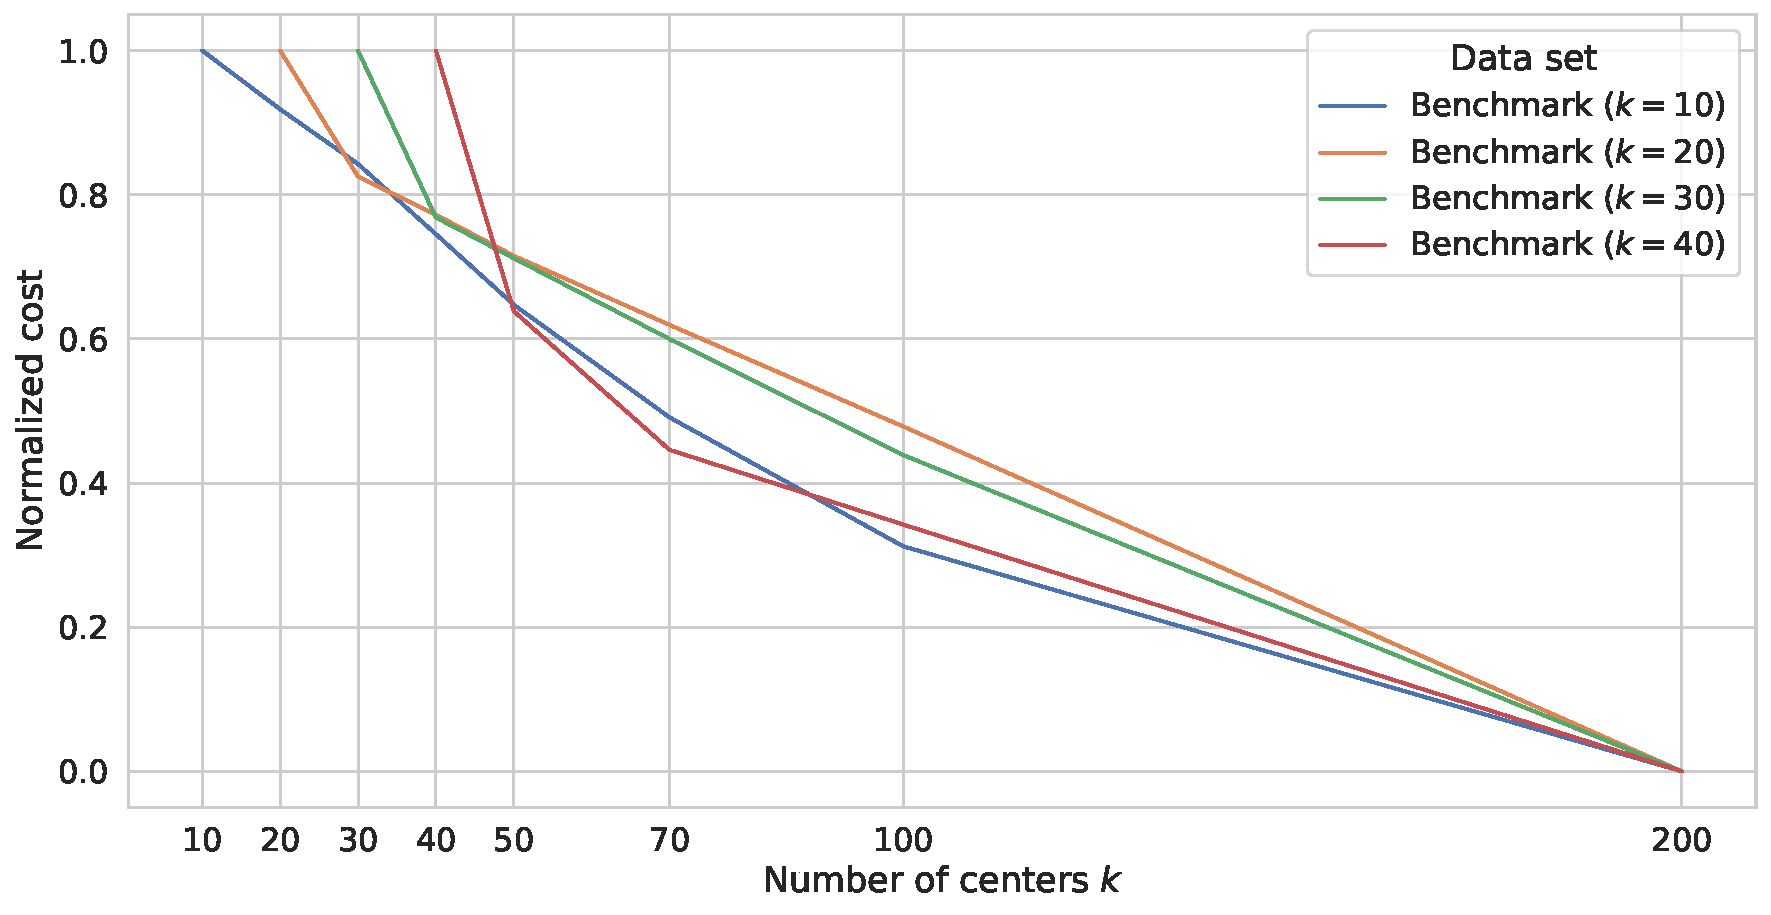
\includegraphics[width=0.9\linewidth]{figures/cost-curves-benchmark.pdf}
  \caption{Shows the clustering costs of four instances of the benchmark framework as a function of the number of centers. In contrast to real-world data sets, the costs do not decrease rapidly as more cluster centers are added.
  }
  \label{fig:cost-curves-benchmark}
\end{figure}

% \begin{figure*}
%  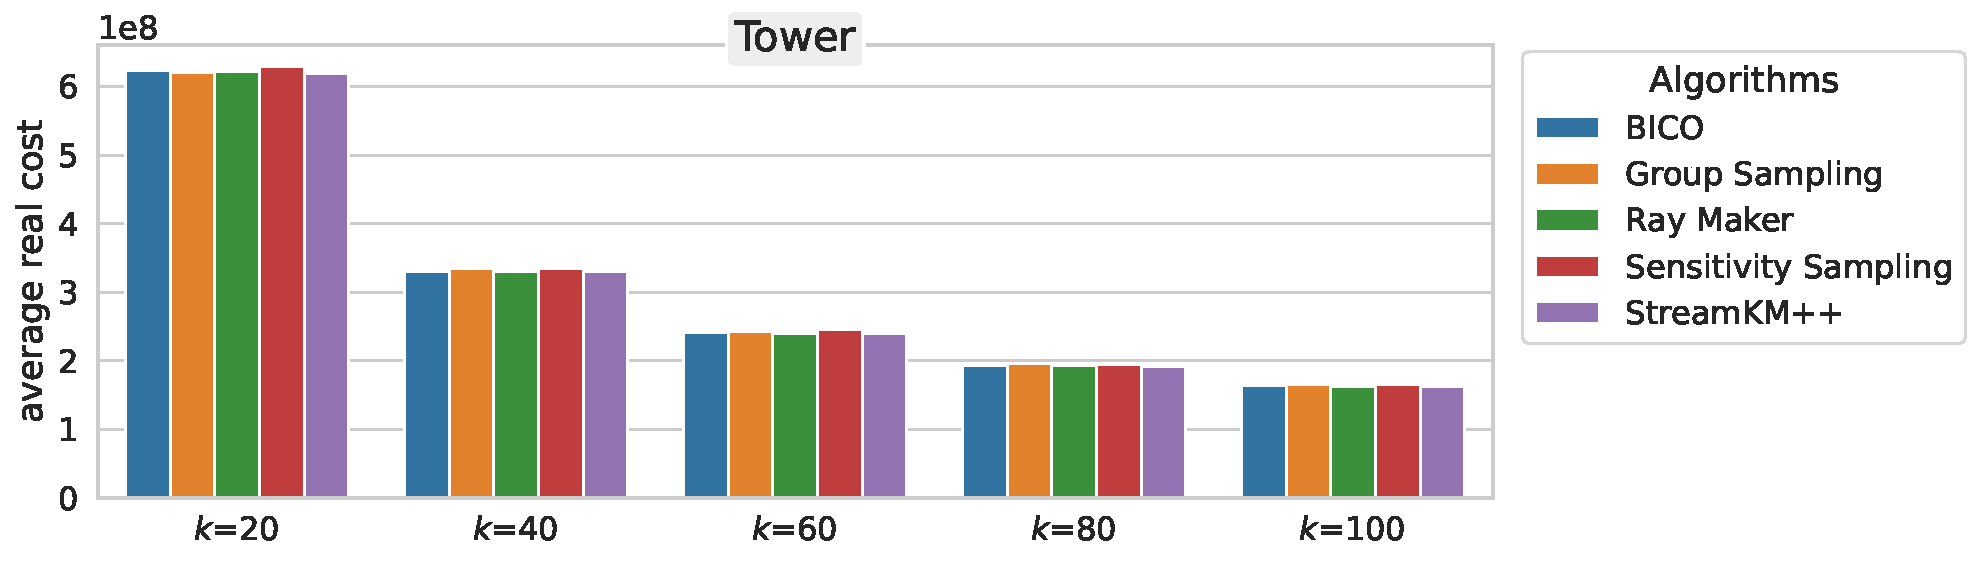
\includegraphics[width=.67\linewidth]{figures/real-costs-Tower.pdf}
%  \newline
%  \subfloat{
%     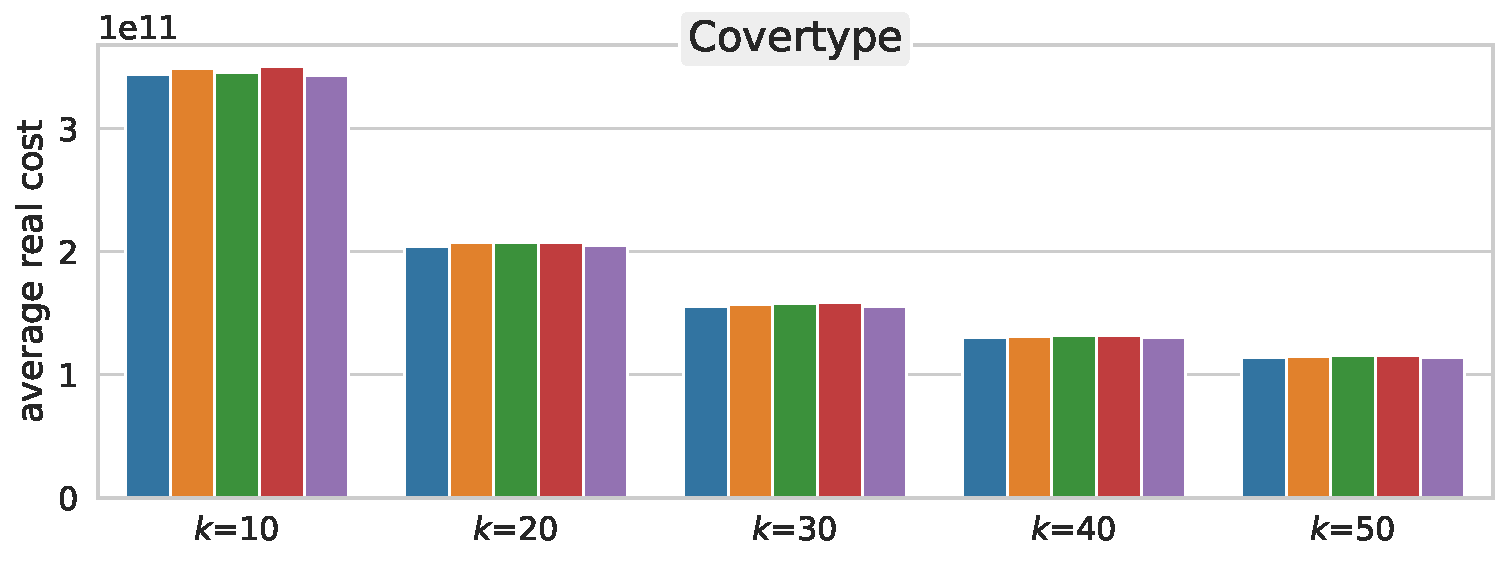
\includegraphics[width=0.5\textwidth]{figures/real-costs-Covertype.pdf}
%  }
%  \subfloat{
%     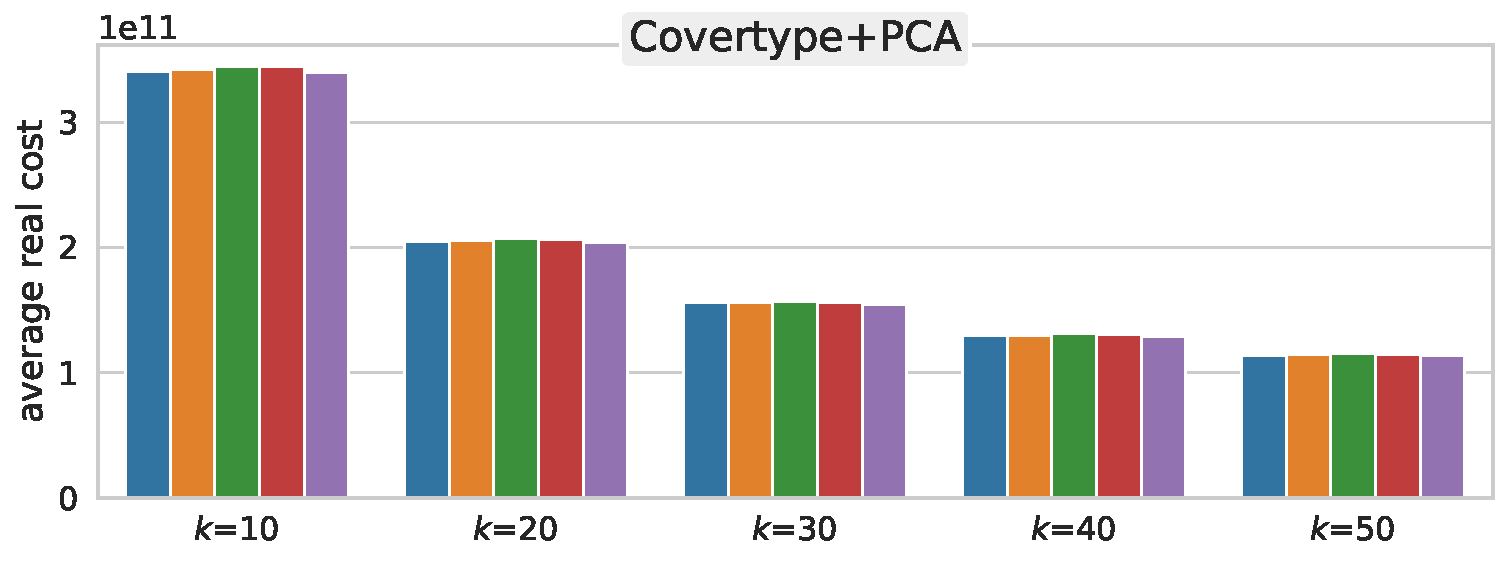
\includegraphics[width=.5\linewidth]{figures/real-costs-Covertype+PCA.pdf}
%  }
%  \newline\newline
%  \subfloat{
%     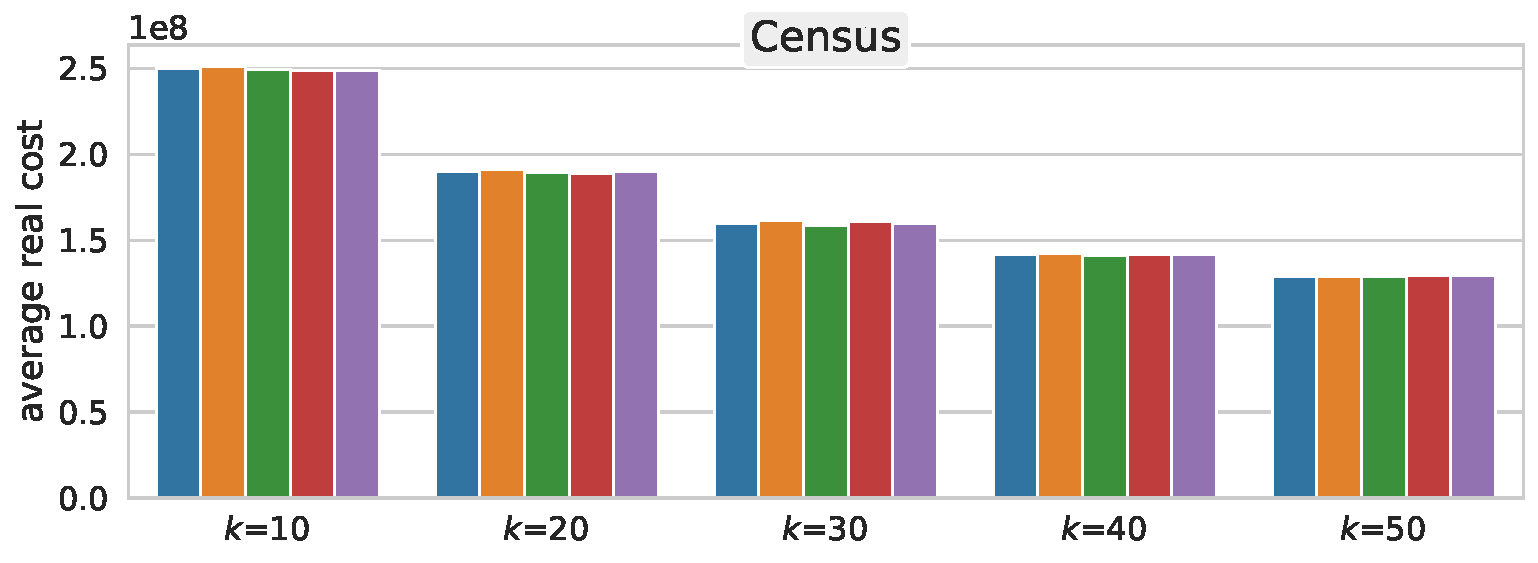
\includegraphics[width=0.5\textwidth]{figures/real-costs-Census.pdf}
%  }
%  \subfloat{
%     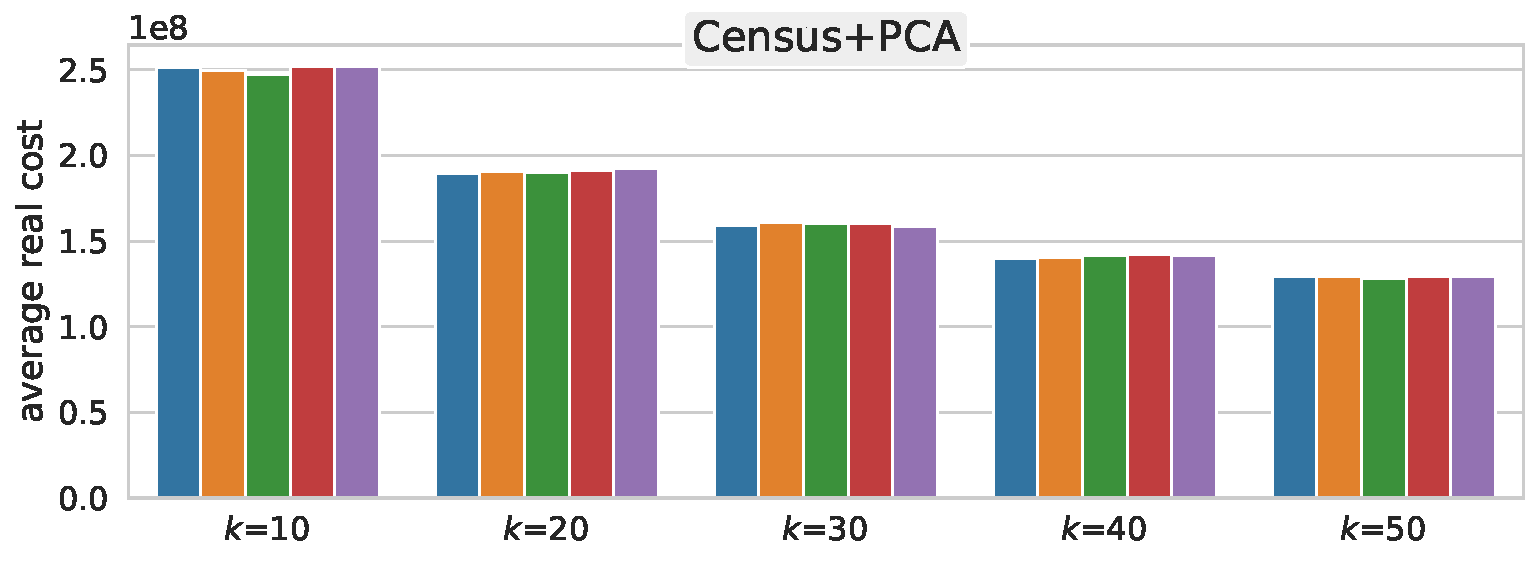
\includegraphics[width=.5\linewidth]{figures/real-costs-Census+PCA.pdf}
%  }
%  \newline\newline
%  \subfloat{
%     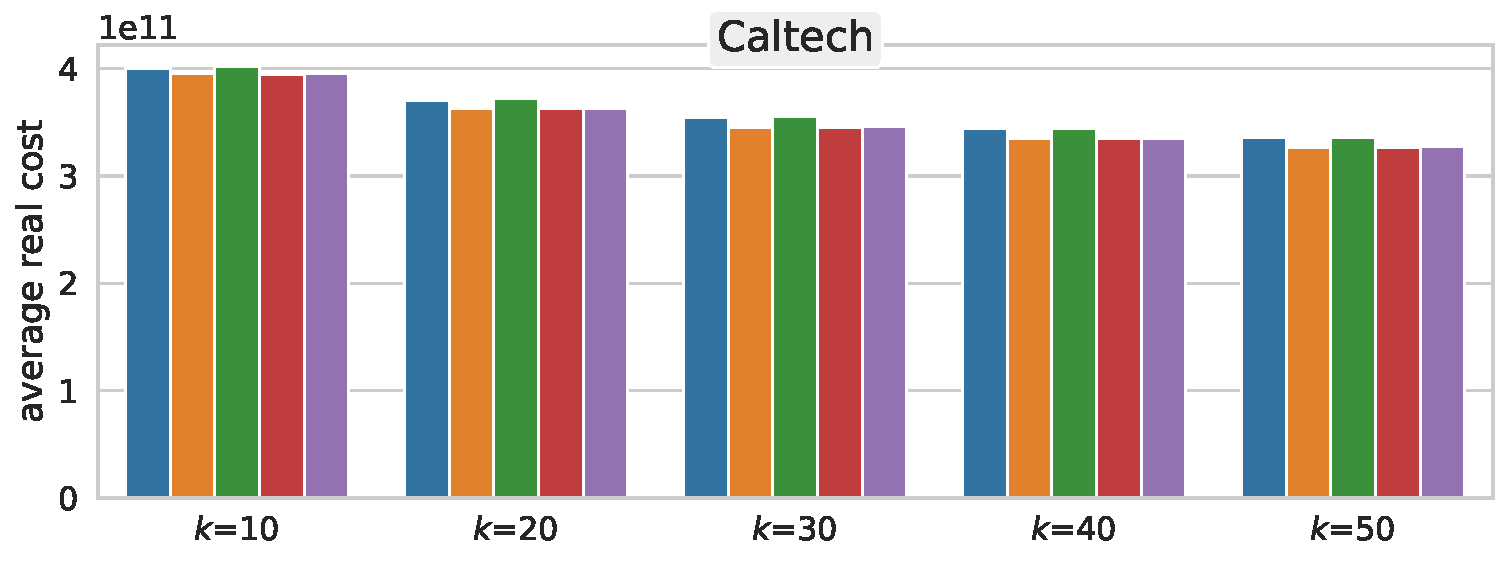
\includegraphics[width=0.5\textwidth]{figures/real-costs-Caltech.pdf}
%  }
%  \subfloat{
%     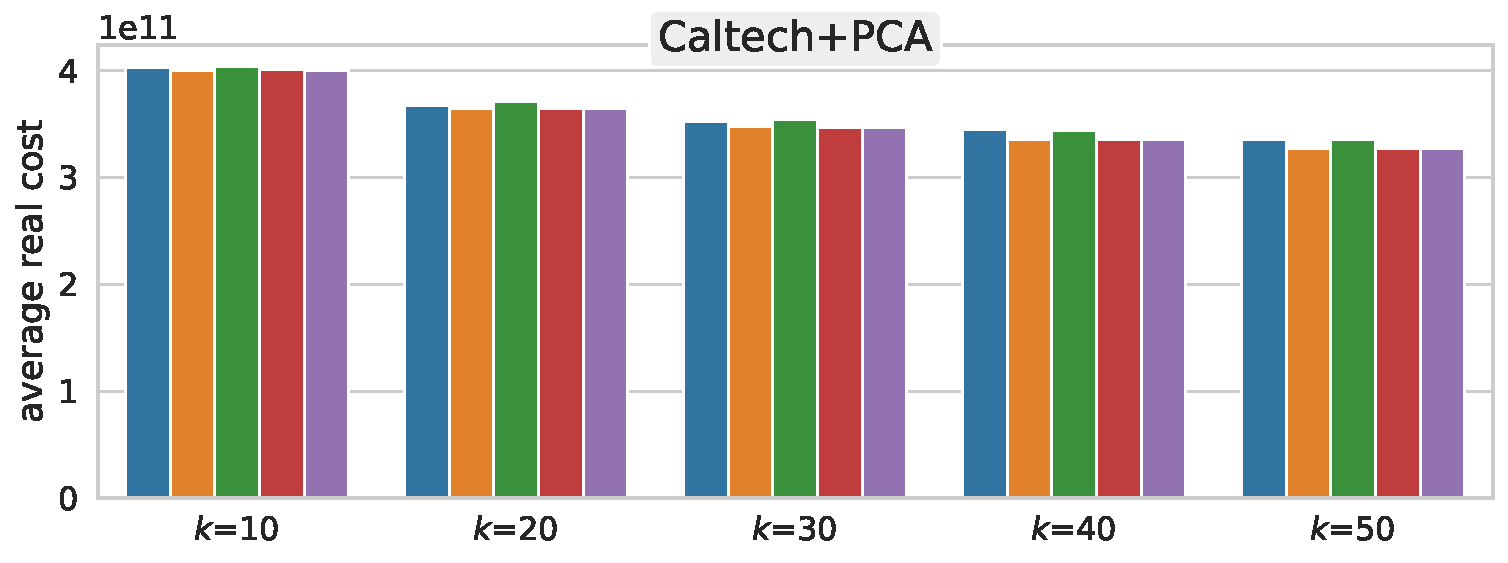
\includegraphics[width=.5\linewidth]{figures/real-costs-Caltech+PCA.pdf}
%  }
%  \newline\newline
%  \subfloat{
%     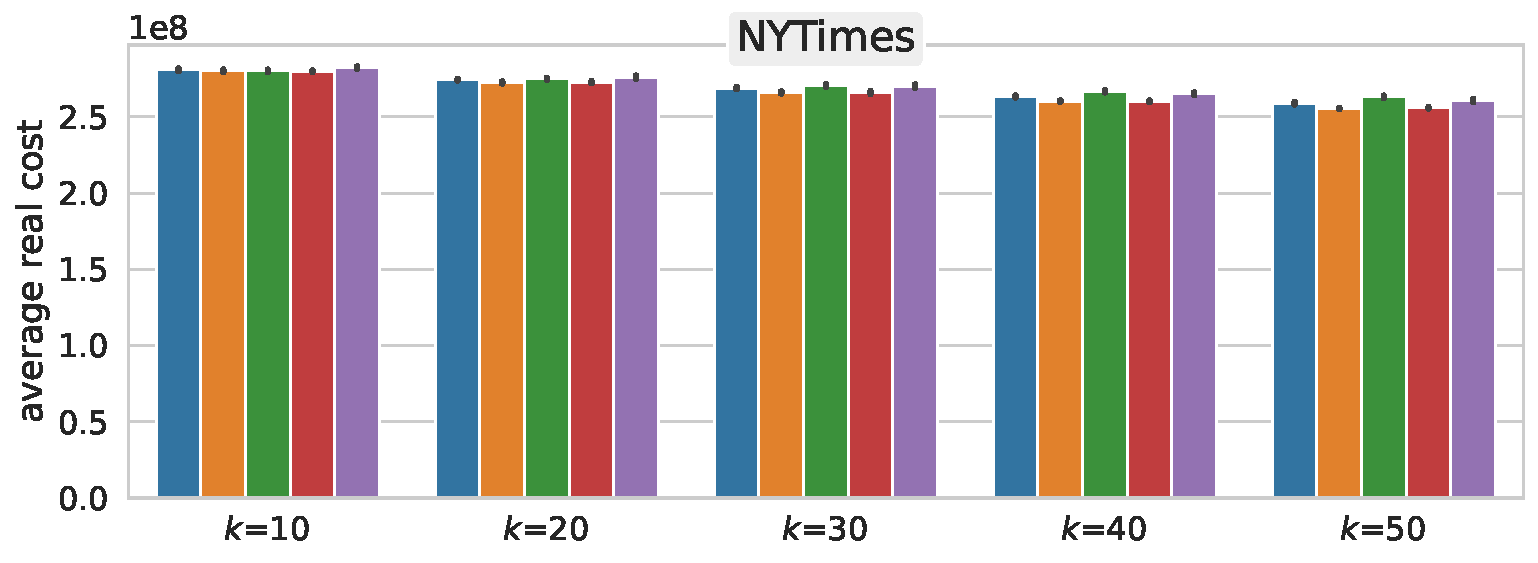
\includegraphics[width=0.5\textwidth]{figures/real-costs-NYTimes.pdf}
%  }
%  \subfloat{
%     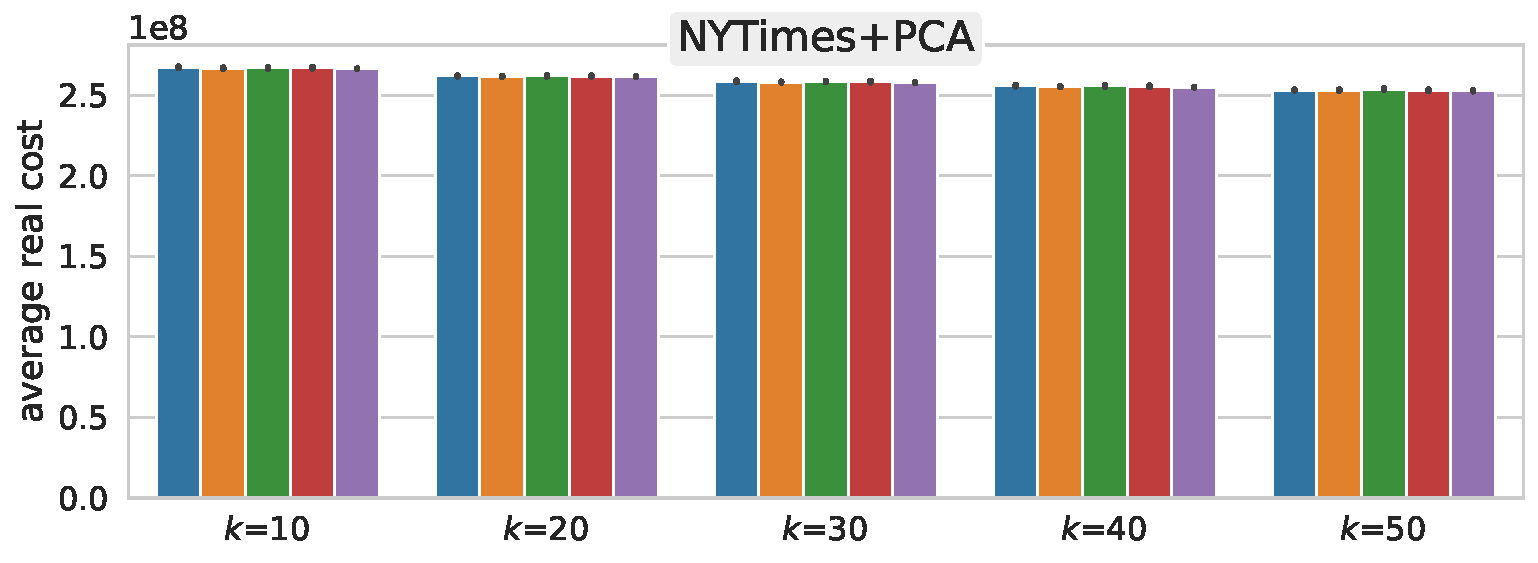
\includegraphics[width=.5\linewidth]{figures/real-costs-NYTimes+PCA.pdf}
%  }
%  \newline\newline
%  \subfloat{
%     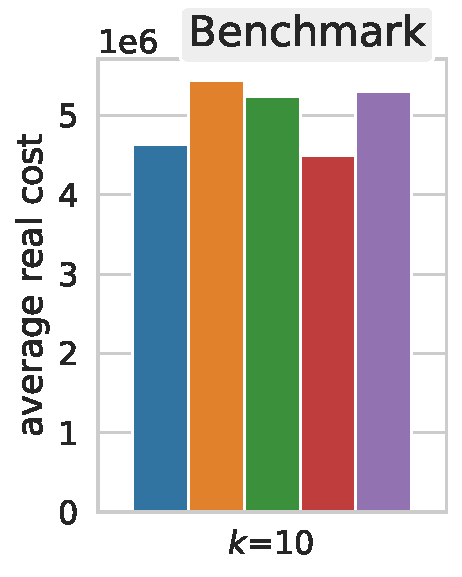
\includegraphics[width=0.15\textwidth]{figures/real-costs-Benchmark-k10.pdf}
%     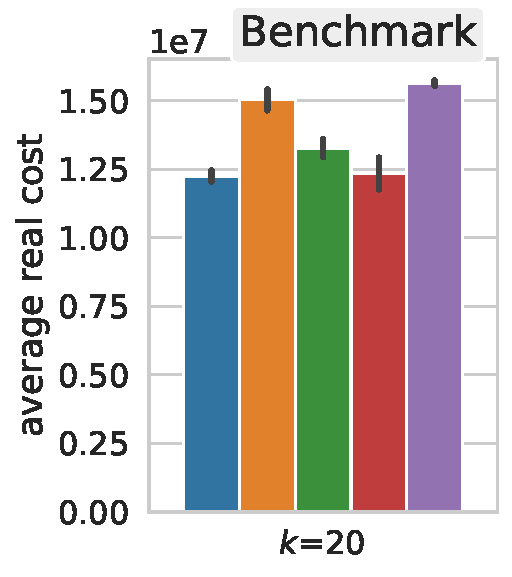
\includegraphics[width=0.165\textwidth]{figures/real-costs-Benchmark-k20.pdf}
%     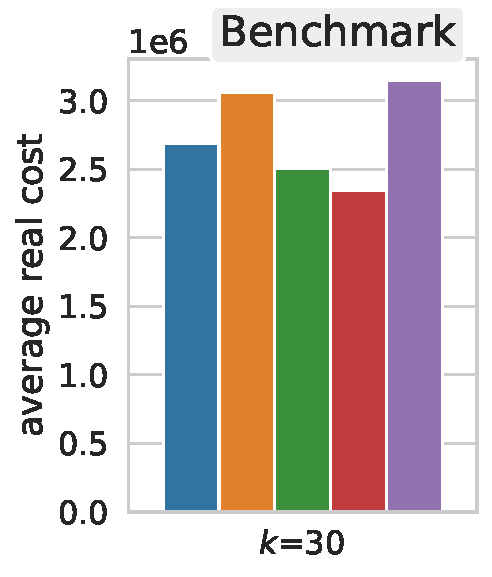
\includegraphics[width=0.16\textwidth]{figures/real-costs-Benchmark-k30.pdf}
%     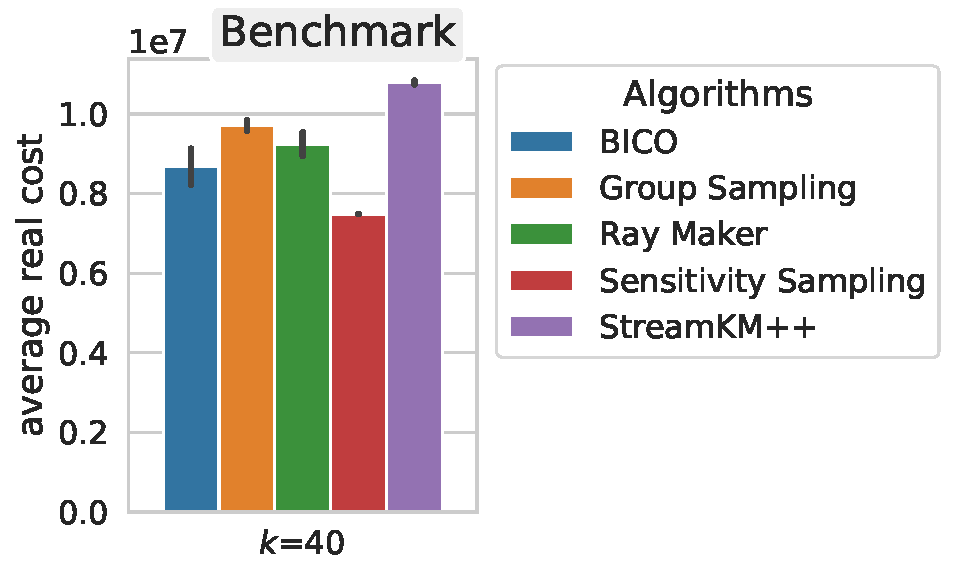
\includegraphics[width=0.31\textwidth]{figures/real-costs-Benchmark-k40.pdf}
%  }
%  \caption{The average costs of running the evaluated coreset algorithms multiple times on different data sets. In general, the five coreset algorithms are able to compute coresets which result in solutions with comparable costs on the different real-world data sets. The differences in cost is more noticeable on the benchmark instances. Here, Senstivity Sampling is the winner because it seems to be better at capturing the correct ``clusters'' inherent in the benchmark instances.}
%  \label{fig:real-costs}
% \end{figure*}



